\section{Games tree}

\begin{example}
    Three politicians are tasked with deciding whether to raise their salaries. 
    The voting is public and happens sequentially. 
    Each politician prefers a salary increase but also wants to vote against it to maintain public support.

    The optimal outcome for each politician is to receive a salary increase while voting against it. 
    The game has the following characteristics:
    \begin{enumerate}
        \item The voting process is sequential, with politicians voting one after another.
        \item Every possible situation is fully known to all players: they are aware of the entire history and all possible future actions.
        \item The final outcome is determined by the majority vote.
    \end{enumerate}
    To represent such a game we can use a tree, where each branch represents a player's vote: a YES vote goes left, and a NO vote goes right. 
    The utilities depend on each player's vote and the final outcome:
    \begin{enumerate} 
        \item YES, but no raise. 
        \item NO, and no raise. 
        \item YES, and a raise. 
        \item NO, and a raise. 
    \end{enumerate}
    The corresponding decision tree looks like this:
    \begin{figure}[H]
        \centering
        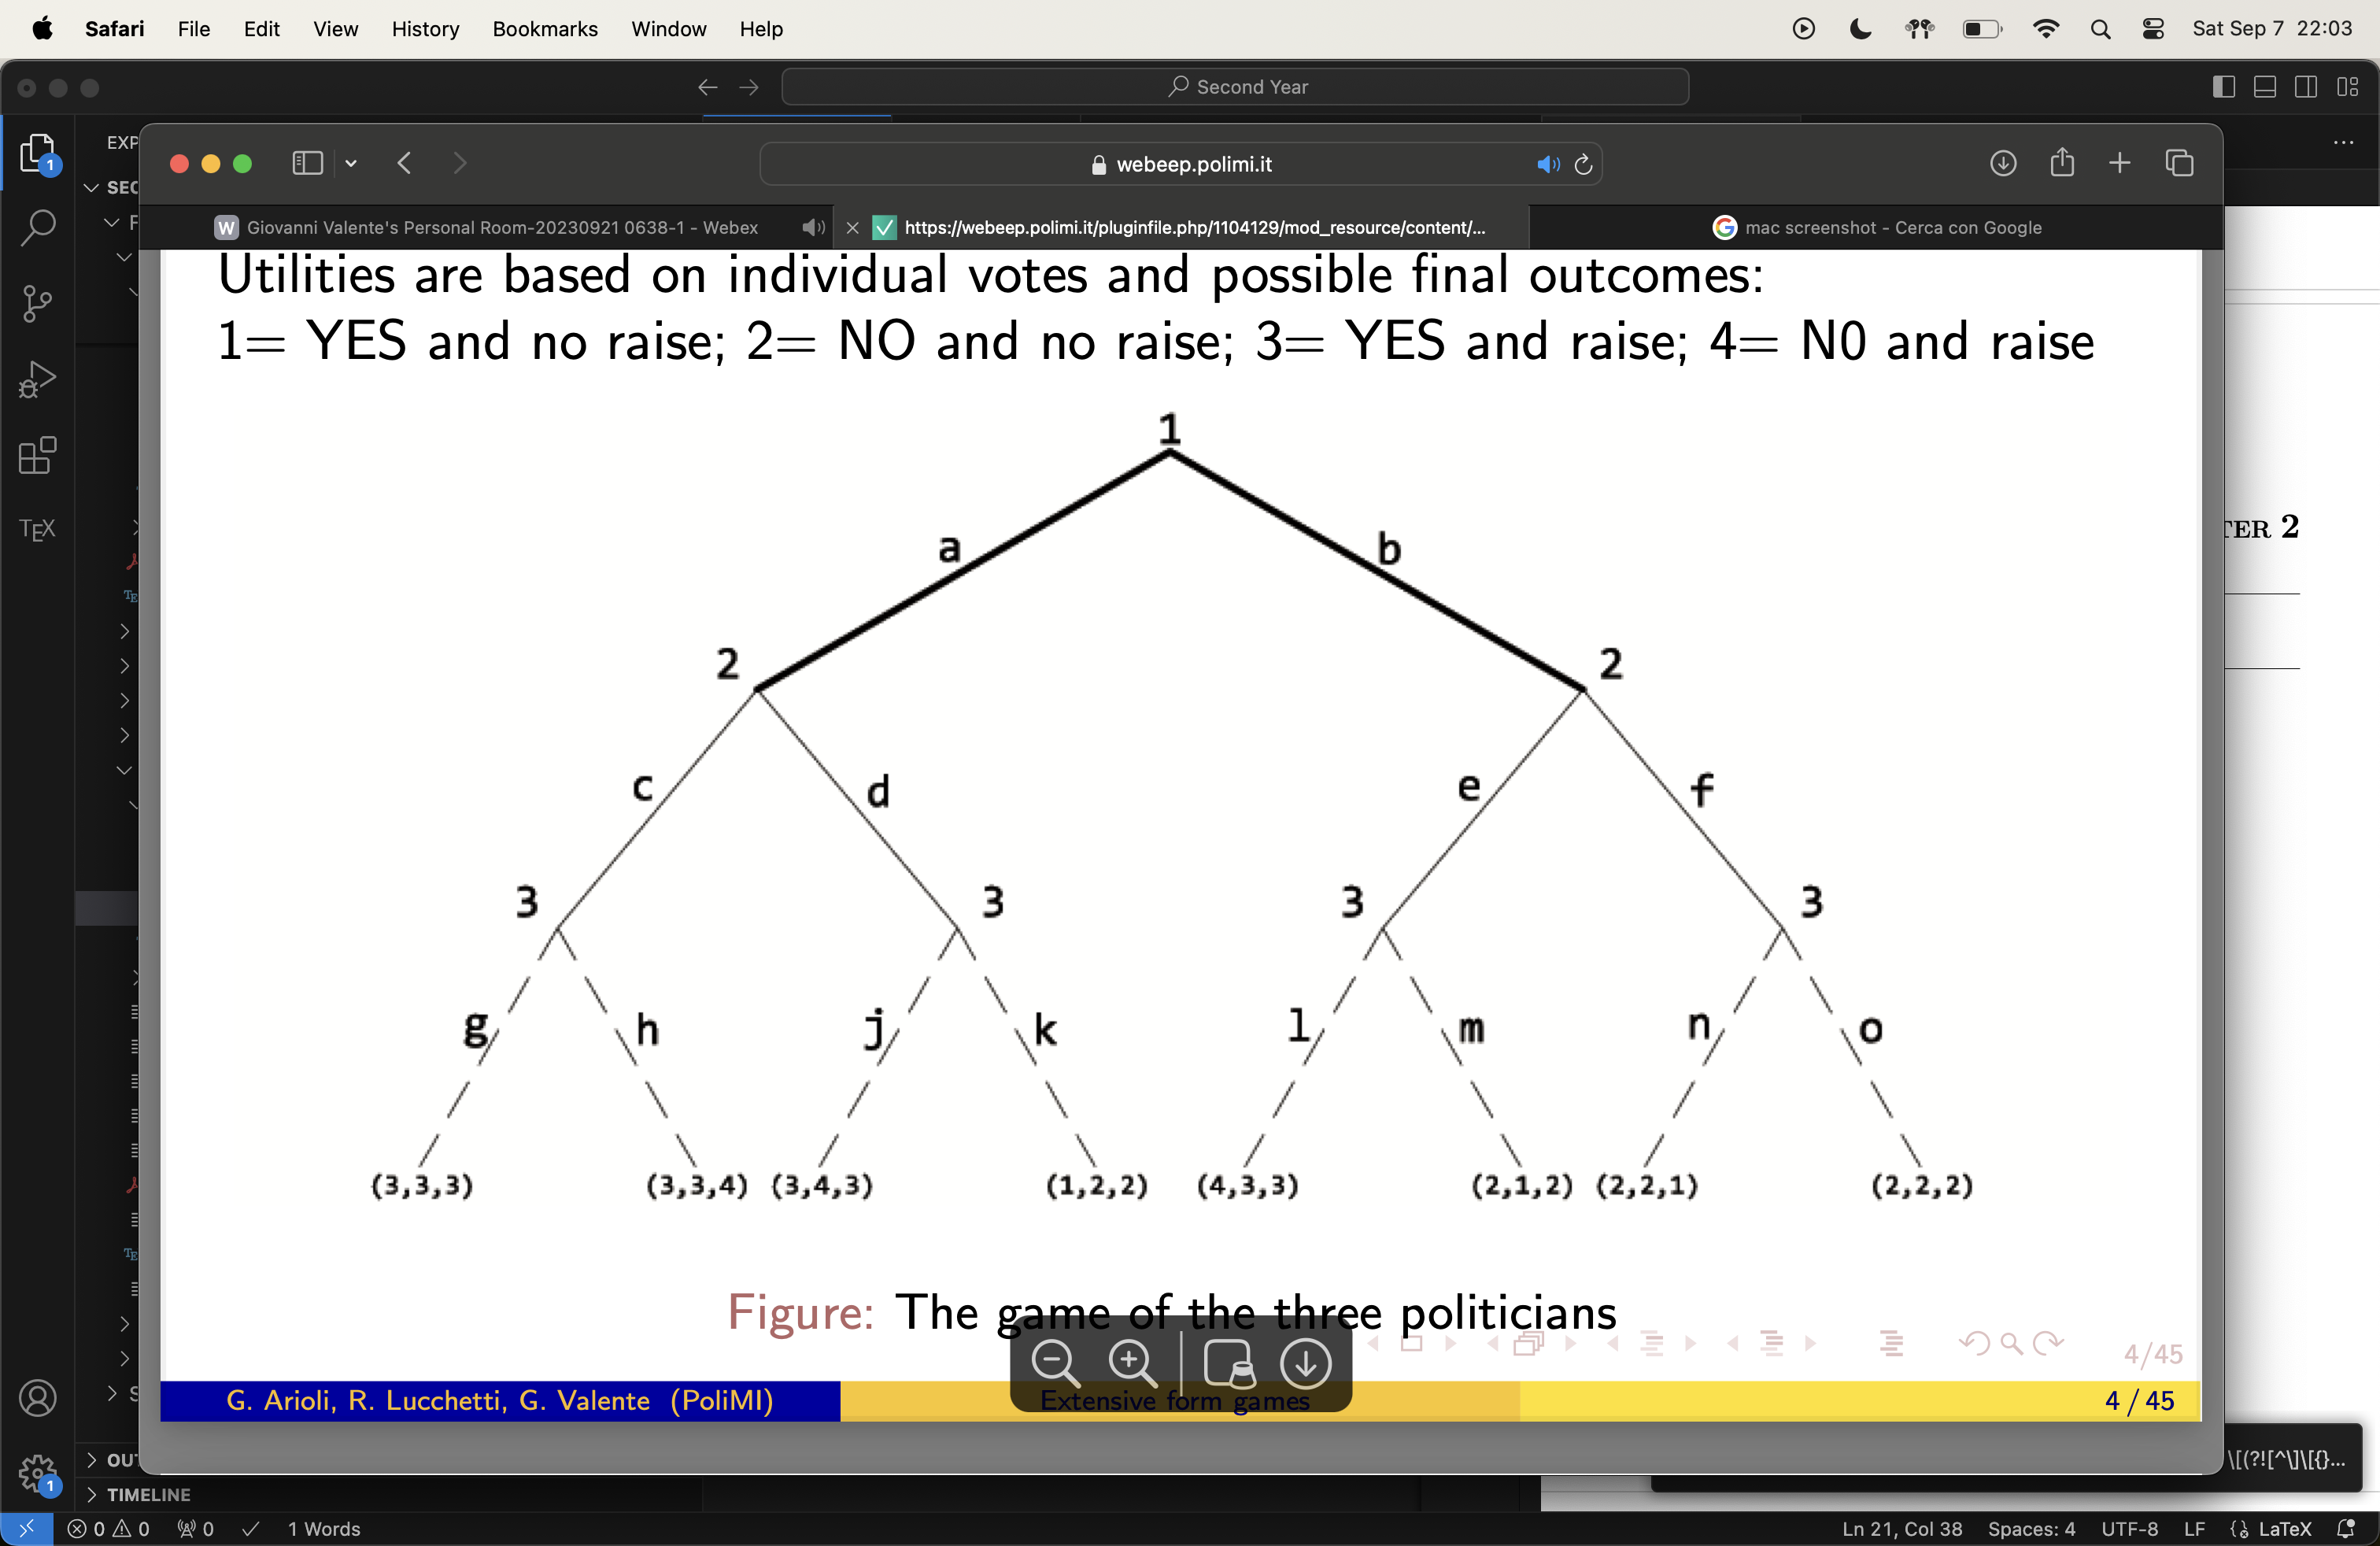
\includegraphics[width=0.75\linewidth]{images/tree.png}
        \caption{Voting game tree}
    \end{figure}
\end{example}
This is an example of a game with perfect information, where each player is fully aware of all prior events.
\begin{example}
    Two players, Player 1 and Player 2, must decide sequentially whether to participate in a game.
    If both choose to play, a coin is flipped (random component $R$): Player 1 wins if it lands heads, and Player 2 wins if it lands tails.
    The corresponding decision tree is as follows:
    \begin{figure}[H]
        \centering
        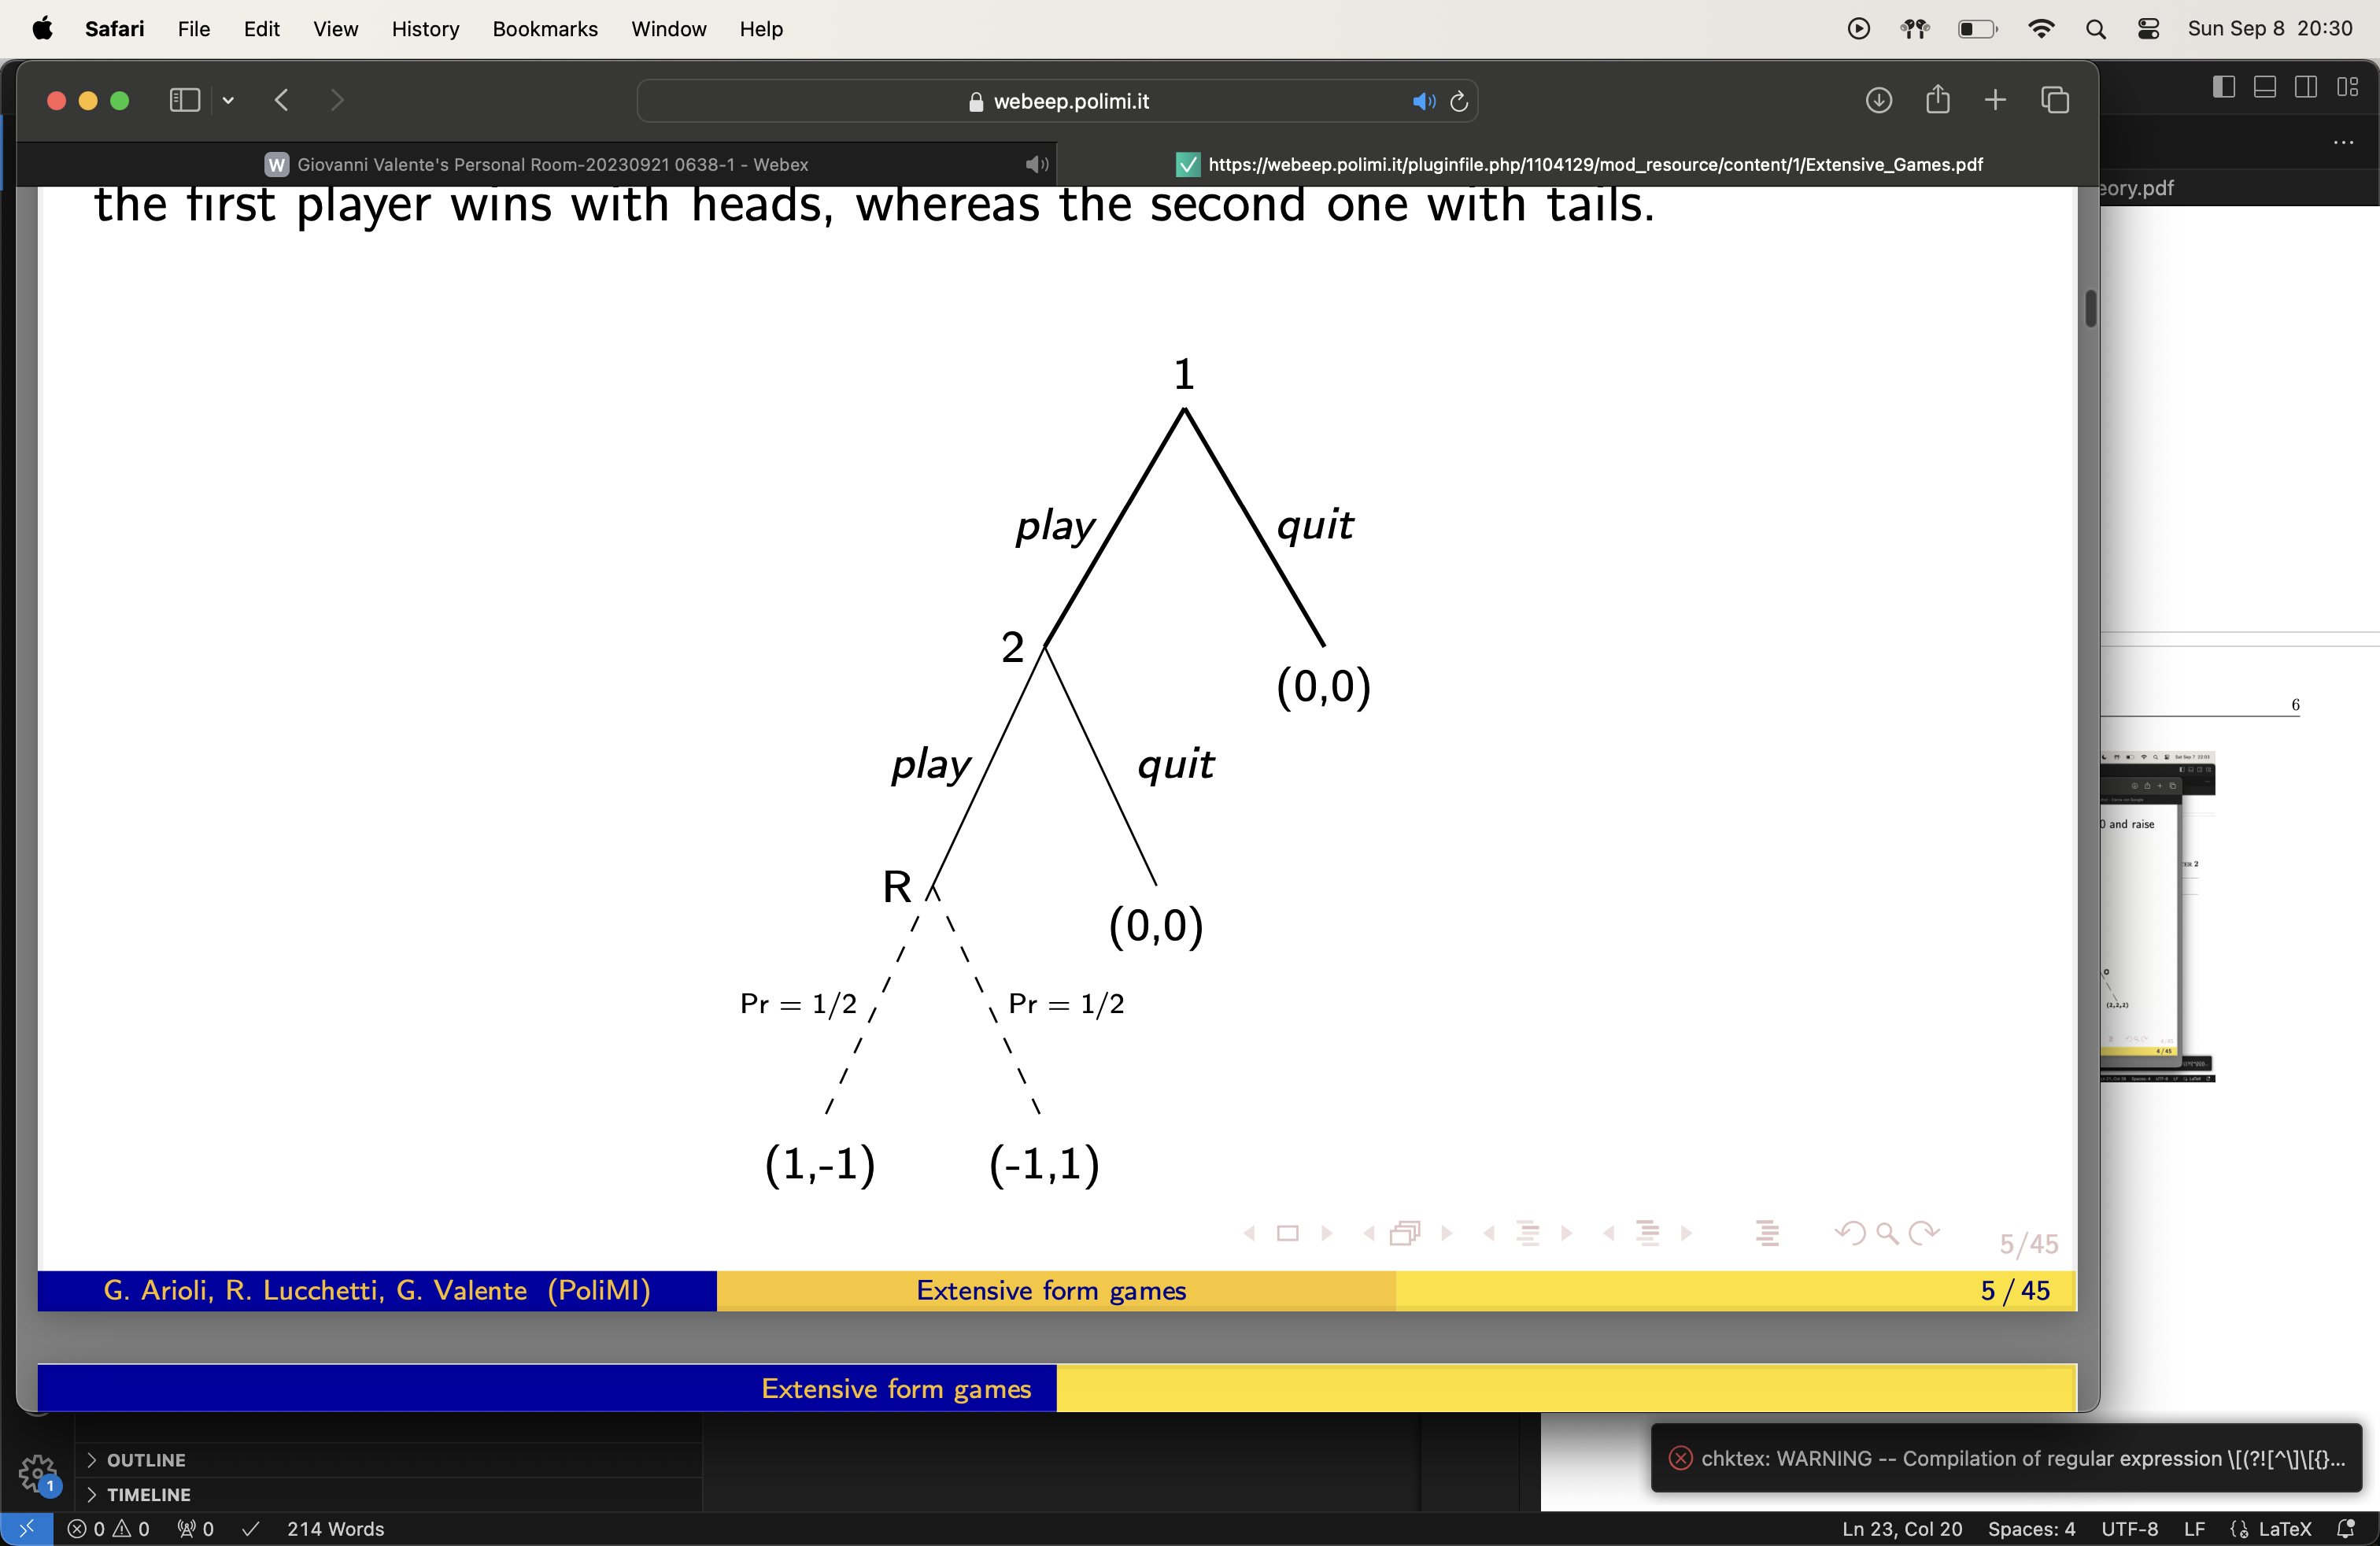
\includegraphics[width=0.75\linewidth]{images/tree1.png}
        \caption{Chance game tree}
    \end{figure}
\end{example}
\begin{definition}[\textit{Finite directed graph}]
    A finite directed graph is a pair $(V,E)$ where:
\end{definition}
\begin{itemize}
    \item $V$ is a finite set, called the set of vertices. 
    \item $E \subset V \times V$ is a set of ordered pairs of vertices, called the directed edges.
\end{itemize}
\begin{definition}[\textit{Path}]
    A path from a vertex $v_1$ to a vertex $v_{k+1}$ is a finite sequence of vertices and edges $v_1,e_1,v_2,\dots,v_k,e_k,v_{k+1}$ such that $e_i \neq e_j$ if $i \neq j$ and $e_j = (v_j,v_{j+1})$. 
\end{definition}
The number $k$ is called the length of the path.
\begin{definition}[\textit{Oriented graph}]
    An oriented graph is a finite directed graph with no bidirectional edges. 
    That is, for all vertices $v_j$ and $v_k$, at most one of $(v_j,v_k)$ and $(v_k,v_j)$ can be an edge in the graph.
\end{definition}
\begin{definition}[\textit{Tree}]
    A tree is a triple $(V,E,x_0)$ where $(V,E)$ is an oriented graph, and $x_0$ is a vertex in $V$ such that there is a unique path from $x_0$ to any other vertex $x \in V$. 
\end{definition}
\begin{definition}[\textit{Child}]
    A child of a vertex $v$ is any vertex $x$ such that $(v,x) \in E$. 
\end{definition}
\begin{definition}[\textit{Leaf}]
    A vertex is called a leaf if it has no children. 
\end{definition}
We say that the vertex $x$ follows the vertex $v$ if there is a path from $v$ to $x$.